% ============================================================================
% BIOMEDICAL / LIFE SCIENCES REVIEW PAPER TEMPLATE
% ============================================================================
% Uses article class with natbib author-year citations (default for biomedical).
% To switch to numbered citations, uncomment \usepackage{cite} and change
% \bibliographystyle to {ieeetr}.
% ============================================================================

\documentclass[11pt,a4paper]{article}

% ---------------------------------------------------------------------------
% CITATION: Author-year (default for biomedical)
% ---------------------------------------------------------------------------
\usepackage[round]{natbib}
% Uncomment for numbered citations:
% \bibliographystyle{ieeetr}

% For author-year:
\bibliographystyle{plainnat}

% ---------------------------------------------------------------------------
% PACKAGES
% ---------------------------------------------------------------------------
\usepackage[utf8]{inputenc}
\usepackage[T1]{fontenc}
\usepackage[margin=2.5cm]{geometry}
\usepackage{enumitem}
\usepackage{amsmath,amssymb,amsfonts}
\usepackage{graphicx}
\usepackage{xcolor}
\usepackage{url}
\usepackage{hyperref}
\hypersetup{colorlinks=true, linkcolor=blue, citecolor=blue, urlcolor=blue}

% Professional tables
\usepackage{booktabs}
\usepackage{longtable}
\usepackage{threeparttable}

% TikZ for pathway maps, mechanism diagrams
\usepackage{tikz}
\usetikzlibrary{
    shapes.geometric, arrows, positioning, fit, backgrounds,
    calc, decorations.pathreplacing, decorations.markings, patterns,
    chains, matrix
}

% Plots
\usepackage{pgfplots}

% Subfigures
\usepackage{subcaption}

% Multi-line comments
\usepackage{comment}

% ---------------------------------------------------------------------------
% COLORS
% ---------------------------------------------------------------------------
\definecolor{primaryblue}{RGB}{55, 110, 180}
\definecolor{secondarygreen}{RGB}{50, 140, 80}
\definecolor{accentorange}{RGB}{230, 130, 30}
\definecolor{highlightred}{RGB}{190, 40, 50}
\definecolor{graytext}{RGB}{100, 100, 100}

% ---------------------------------------------------------------------------
% TITLE PAGE
% ---------------------------------------------------------------------------
\title{[Paper Title — Specific and Descriptive]}

\author{
    [Author 1]\textsuperscript{1,2,*},
    [Author 2]\textsuperscript{1},
    [Author 3]\textsuperscript{3} \\[0.5em]
    \small
    \textsuperscript{1} [Institution 1, Country] \\
    \textsuperscript{2} [Institution 2, Country] \\
    \textsuperscript{3} [Institution 3, Country] \\[0.3em]
    * Correspondence: [email@example.com]
}

\date{}

\begin{document}
\maketitle

% ===========================================================================
% ABSTRACT (200–300 words)
% ===========================================================================
\begin{abstract}
[Summarize:
(1) Background and rationale for the review,
(2) Scope and search methodology (databases searched, inclusion criteria),
(3) Key findings and thematic synthesis,
(4) Clinical/translational implications,
(5) Conclusions and future research priorities.

Be specific. Avoid citations in the abstract.]
\end{abstract}

\vspace{0.5cm}
\noindent\textbf{Keywords:} [Keyword 1]; [Keyword 2]; [Keyword 3]; [Keyword 4]; [Keyword 5]

% ===========================================================================
% 1. INTRODUCTION
% ===========================================================================
\section{Introduction}
[The introduction should:
\begin{itemize}
    \item Establish the clinical or biological significance of the topic
    \item State the burden of disease or prevalence where relevant \citep{ref1}
    \item Identify the knowledge gap this review addresses
    \item Define the review's scope and objectives
    \item Briefly describe the organization of the paper
\end{itemize}

Example: [Disease X] affects approximately [Y] million people worldwide
\citep{who2024report}. Despite recent advances in [area], significant
gaps remain in understanding...]

% ===========================================================================
% 2. DISEASE / CONDITION OVERVIEW
% ===========================================================================
\section{[Disease / Condition] Overview and Clinical Context}
[For disease-focused reviews, provide:
\begin{itemize}
    \item Epidemiology (incidence, prevalence, risk factors) with citations
    \item Clinical presentation and natural history
    \item Current standard of care and its limitations
    \item Unmet clinical needs that motivate the review
\end{itemize}

For basic science reviews, replace with a background on the biological
system or pathway under study.]

\subsection{Epidemiology and Disease Burden}
[Cite key epidemiological studies and global health reports \citep{globalburden2023}.]

\subsection{Current Clinical Management}
[Describe standard diagnosis and treatment. Highlight gaps \citep{guidelines2024}.]

\subsection{Unmet Needs}
[Explicitly state what is missing in current knowledge or practice.]

% ===========================================================================
% 3. MOLECULAR MECHANISMS
% ===========================================================================
\section{Molecular Mechanisms and Pathophysiology}
[This section should synthesize the current understanding of disease mechanisms:
\begin{itemize}
    \item Genetic factors and susceptibility loci \citep{gwas2024}
    \item Signaling pathways and molecular drivers \citep{pathway2023}
    \item Cellular processes (apoptosis, autophagy, inflammation, etc.)
    \item Environmental and epigenetic modifiers
\end{itemize}

Use pathway diagrams (TikZ) to illustrate key mechanisms.

For non-disease reviews, adapt to the relevant mechanistic or theoretical
framework of the field.]

\subsection{Genetic and Epigenetic Factors}
[Summarize key genetic findings and their functional implications.]

\subsection{Signaling Pathways}
[Describe the major pathways involved. A schematic diagram is recommended.]

% Example pathway diagram
\begin{figure}[ht]
    \centering
    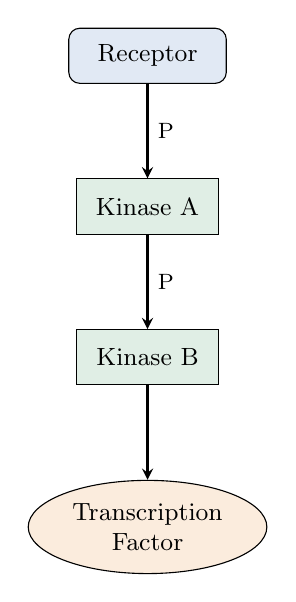
\begin{tikzpicture}[
        node distance=1.2cm,
        receptor/.style={rectangle, draw, fill=primaryblue!15, rounded corners, minimum width=2cm, minimum height=0.7cm, align=center, font=\small},
        kinase/.style={rectangle, draw, fill=secondarygreen!15, minimum width=1.8cm, minimum height=0.7cm, align=center, font=\small},
        tf/.style={ellipse, draw, fill=accentorange!15, minimum width=1.8cm, minimum height=0.7cm, align=center, font=\small},
        arrow/.style={->, >=stealth, thick},
    ]
        \node[receptor] (R) {Receptor};
        \node[kinase, below=of R] (K1) {Kinase A};
        \node[kinase, below=of K1] (K2) {Kinase B};
        \node[tf, below=of K2] (TF) {Transcription\\Factor};

        \draw[arrow] (R) -- (K1) node[midway, right, font=\footnotesize] {P};
        \draw[arrow] (K1) -- (K2) node[midway, right, font=\footnotesize] {P};
        \draw[arrow] (K2) -- (TF);
    \end{tikzpicture}
    \caption{[Pathway description with key components labeled.]}
    \label{fig:pathway}
\end{figure}

% ===========================================================================
% 4. THERAPEUTIC APPROACHES
% ===========================================================================
\section{Therapeutic Approaches}
[Organize by therapeutic modality or target class:
\begin{itemize}
    \item Small molecule inhibitors \citep{drug2024}
    \item Biologics and monoclonal antibodies \citep{mab2023}
    \item Gene therapies and nucleic acid therapeutics \citep{gene2024}
    \item Cell-based therapies \citep{cell2023}
    \item Combination strategies
\end{itemize}

For each approach, discuss:
\begin{itemize}
    \item Mechanism of action
    \item Key preclinical and clinical evidence
    \item Efficacy and safety profile
    \item Limitations and resistance mechanisms
\end{itemize}]

\subsection{Small Molecule Approaches}
[Discuss key drug classes, representative compounds, and clinical data.]

\subsection{Biologics and Antibody-Based Therapies}
[Cover monoclonal antibodies, antibody-drug conjugates, bispecifics, etc.]

\subsection{Gene and Cell Therapies}
[Discuss viral vectors, CRISPR-based approaches, CAR-T, stem cell therapies.]

\subsection{Combination Strategies}
[Rationale, preclinical evidence, and clinical trials for combination approaches.]

% Example clinical trial summary table
\begin{table}[ht]
\centering
\caption{Key clinical trials of [therapeutic class].}
\label{tab:trials}
\begin{tabular}{lllll}
\toprule
\textbf{Trial} & \textbf{Phase} & \textbf{N} & \textbf{Primary Endpoint} & \textbf{Ref} \\
\midrule
Trial A & III & 450 & PFS (HR 0.62) & \citep{trial2024} \\
Trial B & II & 120 & ORR 48\% & \citep{trial2023} \\
Trial C & III & 600 & OS (HR 0.71) & \citep{trial2024b} \\
\bottomrule
\end{tabular}
\end{table}

% ===========================================================================
% 5. CLINICAL TRANSLATION
% ===========================================================================
\section{Clinical Translation and Trials}
[Synthesize evidence from clinical studies:
\begin{itemize}
    \item Phase I–III trial results for key therapies
    \item Biomarker-driven patient selection
    \item Pharmacokinetics and pharmacodynamics
    \item Toxicity management
    \item Real-world evidence and post-marketing data
\end{itemize}

Consider using forest plots or summary tables for meta-analyses.]

\subsection{Completed Trials and Key Findings}
[Summarize the most practice-changing trial results.]

\subsection{Biomarker Development}
[Discuss predictive and prognostic biomarkers.]

\subsection{Regulatory Landscape}
[FDA/EMA approvals, guidelines, and reimbursement considerations.]

% ===========================================================================
% 6. FUTURE PERSPECTIVES
% ===========================================================================
\section{Future Perspectives and Emerging Directions}
[Forward-looking synthesis:
\begin{itemize}
    \item Next-generation therapies in the pipeline
    \item Emerging technologies (single-cell, spatial omics, AI/ML applications)
    \item Unresolved biological questions
    \item Trial design innovations (basket/umbrella trials, adaptive designs)
    \item Personalized medicine approaches
\end{itemize}]

\subsection{Emerging Technologies}
[Discuss how new technologies may transform the field.]

\subsection{Key Unanswered Questions}
[List the most important open questions that should guide future research.]

% ===========================================================================
% 7. CONCLUSION
% ===========================================================================
\section{Conclusion}
[Concise summary of the review:
\begin{itemize}
    \item Restate the significance of the topic (1 sentence)
    \item Summarize 2–3 key thematic findings
    \item State the most important clinical or translational implication
    \item End with a forward-looking statement on future priorities
\end{itemize}

Do not introduce new information or citations here.]

% ===========================================================================
% ACKNOWLEDGEMENTS
% ===========================================================================
\section*{Acknowledgements}
[Acknowledge funding sources, colleagues, and any conflicts of interest.]

% ===========================================================================
% BIBLIOGRAPHY
% ===========================================================================
% For author-year (default with natbib):
\bibliographystyle{plainnat}

% For numbered citations, uncomment the line below and change the style above:
% \bibliographystyle{ieeetr}

\bibliography{ref}

\end{document}
